% CARICA IL LAYOUT PER IL DOCUMENTO
\documentclass[11pt,a4paper]{article}
\usepackage[a4paper,portrait,top=3.5cm,bottom=3.5cm,left=3cm,right=3cm,bindingoffset=5mm]{geometry}
\usepackage[T1]{fontenc}
\usepackage[utf8x]{inputenc}
\usepackage{graphicx}
\usepackage{caption}
\usepackage[italian]{babel}
\usepackage{listings}
\usepackage{fancyhdr}
\usepackage{lastpage}
\usepackage{hyperref}
\usepackage{array,booktabs}
\usepackage{subcaption}

% Identazione tabella gruppo Frontespizio.tex
\newcolumntype{L}[1]{>{\raggedright\let\newline\\\arraybackslash\hspace{0pt}}m{#1}}
\newcolumntype{C}[1]{>{\centering\let\newline\\\arraybackslash\hspace{0pt}}m{#1}}
\newcolumntype{R}[1]{>{\raggedleft\let\newline\\\arraybackslash\hspace{0pt}}m{#1}}

% Header and Footer

\fancypagestyle{std}{
	\fancyhf{}
	\lhead{
\includegraphics[width=1.7cm]{images/frontImage.png}}
	\chead{}
	\rhead {\nouppercase{\leftmark}}
	\lfoot{}
	\cfoot{}
	\rfoot{Pagina \thepage\ di \pageref{LastPage}}
	\renewcommand{\headrulewidth}{0.3pt}
	\renewcommand{\footrulewidth}{0.3pt}
}

\fancypagestyle{romano}{
	\fancyhf{}
	\lhead{
\includegraphics[width=1.7cm]{images/frontImage.png}}
	\chead{}
	\lfoot{}
	\cfoot{}
	\rfoot{}
	\rfoot{\thepage}
	\renewcommand{\headrulewidth}{0.3pt}
	\renewcommand{\footrulewidth}{0.3pt}
}
	
% DEFINIZIONE ELEMENTI FRONTESPIZIO
\title{\bfseries Scherma Castelfranco Veneto}
\author{Chiara Bigarella mat. 1008533\\Pavanello Mirko mat. 1009424 \\Massimiliano Sartoretto mat. 1008168,\\ Paolo Tesser mat. 1026527}
\date{A.A. 2013/2014}
\begin{document}
%\maketitle
%\vspace {20 mm}
%
\includegraphics[width=150mm, height=120mm]{images/page_logo.png}
\begin{titlepage}
 \begin{center}
     
\includegraphics[width=8cm]{images/page_logo.png}\\
     
     \vspace{3em} \hrule \vspace{2em}
     {\LARGE \LARGE \LARGE \textbf{Scherma Castelfranco Veneto}}\\
     \vspace{2em} \hrule \vspace{2em}
     \vspace{2em}
 \end{center}

\begin{center}
	{\LARGE { \scshape gruppo L'intrusa}}\\
	\vspace{2em}
    \begin{tabular}{ R{5cm} | L{5cm}  }
    \textbf{Chiara Bigarella} & mat. 1008533\\ \\
    \textbf{Mirko Pavanello} & mat. 1009424 \\ \\
    \textbf{Massimiliano Sartoretto} & mat. 1008168 \\ \\
    \textbf{Paolo Tesser} &  mat. 1026527 \\ \\
    \end{tabular}
\end{center}

\vskip 0.7cm
\begin{center}
Sommario: \\Relazione del progetto di Tecnologie Web AA 2013-14\\
\end{center}
\end{titlepage}
\newpage


% INDICI DI CONTENUTO E IMMAGINI
\pagestyle{romano}
\pagenumbering{Roman}
\newpage
	\tableofcontents
	\listoffigures
\newpage
\pagenumbering{arabic}
\pagestyle{std}

% CORPO DEL DOCUMENTO

\newpage
\section{Accesso al sito}
	Il sito \`e accessibile all'indirizzo web \href{http://tecnologie-web.studenti.math.unipd.it/tecweb/~ptesser/}{http://tecnologie-web.studenti.math.unipd.it/tecweb/~ptesser/}.

\subsection{Amministrazione}
La parte amministrativa \`e accessibile attraverso il link \textit{Area privata} presente in ogni pagina del sito. \\ I dati di accesso sono:
\begin{itemize}
	\item \textbf{username}: admin
	\item \textbf{password}: admin
\end{itemize}
Email del referente: p.tesser921@gmail.com

\section{Descrizione generale}
	Il gruppo ha deciso di realizzare un sito di pubblicazione di articoli e documenti, per la societ\`a sportiva di scherma di Castelfranco Veneto. L'applicativo web di questa associazione esiste gi\`a, ma non \`e conforme alle regole del W3C e non \`e accessbile. Inoltre l'inserimento degli articoli e dei documenti veniva fatto direttamente da codice senza l'ausilio di database esterni e senza strumenti per l'inserimento di dati.
Il permesso di utilizzare i contenuti gi\`a esistenti ci \`e stato fornito dal Presidente e dal gestore del sito.
\\L'applicativo sar\`a composto da una parte utente, accessibile da chiunque, e una parte amministratore, accessibile solamente dalla persona incaricata di pubblicare articoli e documenti. 
Per un utente del sito sar\`a dunque possibile consultare gli articoli recenti, scaricare documenti in formato PDF, e accedere a informazioni pubbliche della societ\`a, mentre l'amministratore potr\`a accedere all'area privata e gestire le risorse pubblicate, inserendo, modificando o eliminando articoli e/o documenti.\\


	
\newpage
\section{Progettazione}
	\subsection{Struttura}
		\subsubsection{Repository}
	La cartella del progetto \`e stata organizzata nelle seguenti cartelle:
	\begin{itemize}
		\item {\bfseries public\_html} che contiene le pagine statiche, gli stili e gli script javaScript.
		\item {\bfseries data} che contiene i documenti accessibili solo internamente al server, quindi i file xml, i fogli di trasformazione, la definizione degli schemi e le pagine html private che vengono usate da Perl per comporre pagine dinamiche. Limitiamo cos\`i al massimo il rischio di intrusioni.
		\item {\bfseries cgi-bin} che contiene gli script scritti in Perl.
	\end{itemize}
\subsubsection{Definizione}
	\noindent La parte \underline{utente} \`e composta da 7 pagine:
\begin{itemize}
	\item {\bfseries\textit{Articoli.cgi}} mostra gli articoli recentemente inseriti. Ne rende disponibili 5 al primo caricamento, e attraverso un link “mostra altri“ permette di visualizzarne un numero sempre superiore. Uno script javascript si occupa di creare un'ancora sull'ultimo articolo visionato in modo da non causare disorientamento.
	\item {\bfseries\textit{Documenti.cgi}} mostra i documento scaricabili con una breve descrizione. Ad ogni documento \`e associata l'estensione del file e la dimensione, in modo da dare all'utente pi\`u informazioni sul download.
	\item {\bfseries\textit{Storia.html}} pagina statica che descrive la storia della societ\`a.
	\item {\bfseries\textit{Staff.html}} pagina statica che mostra le persone che fanno parte dello staff.
	\item {\bfseries\textit{Corsi.html}} pagina statica che mostra l'orario dei corsi.
	\item {\bfseries\textit{amministra.cgi}} mostra un form di login per l'accesso all'area privata.
\end{itemize}

La parte \underline{amministratore} \`e composta da 6 pagine:
\begin{itemize}
	\item {\bfseries\textit{InserisciArticolo.cgi}} permette di inserire un nuovo articolo. In questa pagina \`e presente un form di inserimento, con dei bottoni che permettono di inserire il testo formattato attraverso dei tag html. Poich\`e l'amministratore ha interesse nel rendere accessibili i propri contenuti, sar\`a aiutato dall'editor per descrivere in maniera opportuna tutte le parole che inserisce. Nel caso javaScript sia disabilitato scompaiono i bottoni e appare una breve guida sui tag disponibili.
	\item {\bfseries\textit{ModificaArticolo.cgi}} che permette di scegliere un articolo da modificare e lo ripresenta in un form di modifica.
	\item {\bfseries\textit{EliminaArticolo.cgi}} che permette di selezionare uno o pi\`u articoli da eliminare.
	\item {\bfseries\textit{InserisciDocumento.cgi}} che permette di inserire un nuovo documento attraverso un form, dal quale \`e possibile inserire un titolo, una breve descrizione e il documento stesso.
	\item {\bfseries\textit{ModificaDocumento.cgi}} permette di scegliere un documento da modificare, e lo ripresenta in un form di modifica.
	\item {\bfseries\textit{EliminaDocumento.cgi}}  permette di selezionare uno o pi\`u documenti da eliminare.
\end{itemize}

	Tutte queste pagine sono dinamiche, create attraverso lo script perl \textit{amministraSezionePrivata.cgi} che si occupa di delegare alle funzioni la composizione delle pagine html da dare in output.
	
\subsubsection{Database}
	La persistenza dei data \`e ottenuta attraverso due file XML validi secondo gli schemi definiti in \textit{articoli.xsd} e \textit{documenti.xsd}. Si \`e scelto XML Schema poich\`e garantisce l'espressivit\`a di cui abbiamo bisogno, in particolare per avere a disposizione i tipi primitivi date e anyURI, utili nella definizione di articoli e documenti.
	\subsection{Presentazione}
		Il sito propone un layout a schede, poich\`e il numero di pagine \`e relativamente basso e non riteniamo che in futuro possa aumentare il numero di voci del men\`u.
Abbiamo previsto tre layout differenti basati sulla dimensione dello schermo del device. 
\begin{itemize}
	\item Uno per dispositivi {\bfseries desktop}, disponibile per schermi sopra gli 850 pixel di larghezza.
	\item Uno per dispositivi {\bfseries tablet}, disponibile per schermi dai 480 ai 850 pixel di larghezza.
	\item Uno per dispositivi {\bfseries mobile}, disponibile per schermi fino ai 480 pixel di larghezza.
\end{itemize}


%\begin{figure}[h]
%        \centering
%        \begin{subfigure}[b]{0.10\textwidth}
%		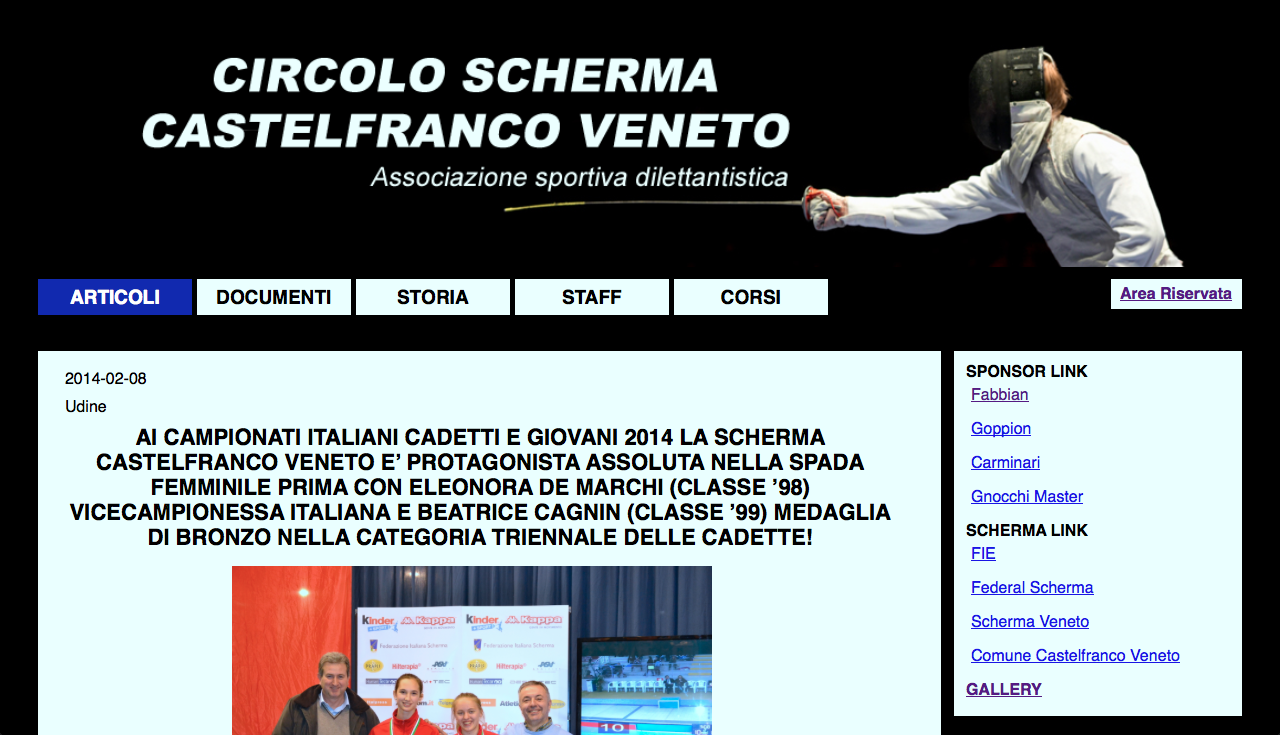
\includegraphics[scale=0.32]{images/articoli_desktop.png}
%		\caption{Screenshot desktop articoli.cgi}
%        \end{subfigure}
%        ~
%        \begin{subfigure}[b]{0.10\textwidth}
%		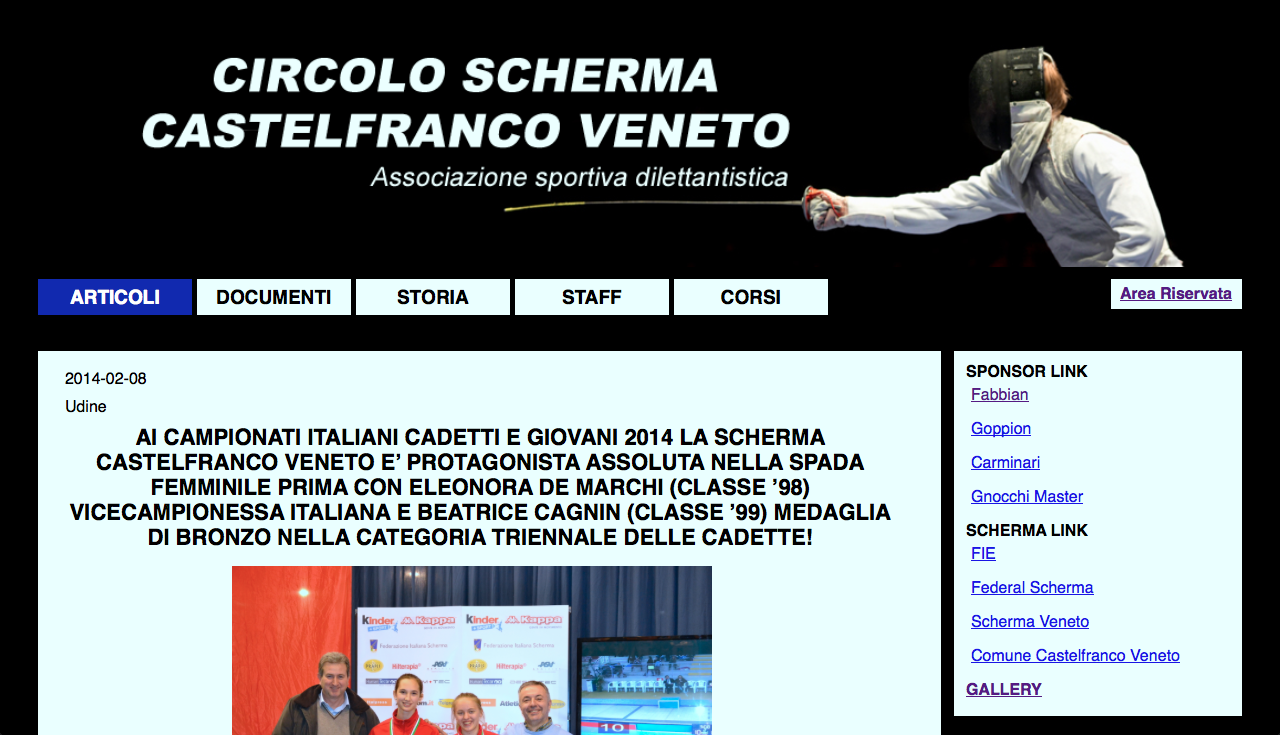
\includegraphics[scale=0.30]{images/articoli_tablet.png}
%		\caption{Screenshot tablet articoli.cgi}
%        \end{subfigure}
%        ~
%        \begin{subfigure}[b]{0.30\textwidth}
%		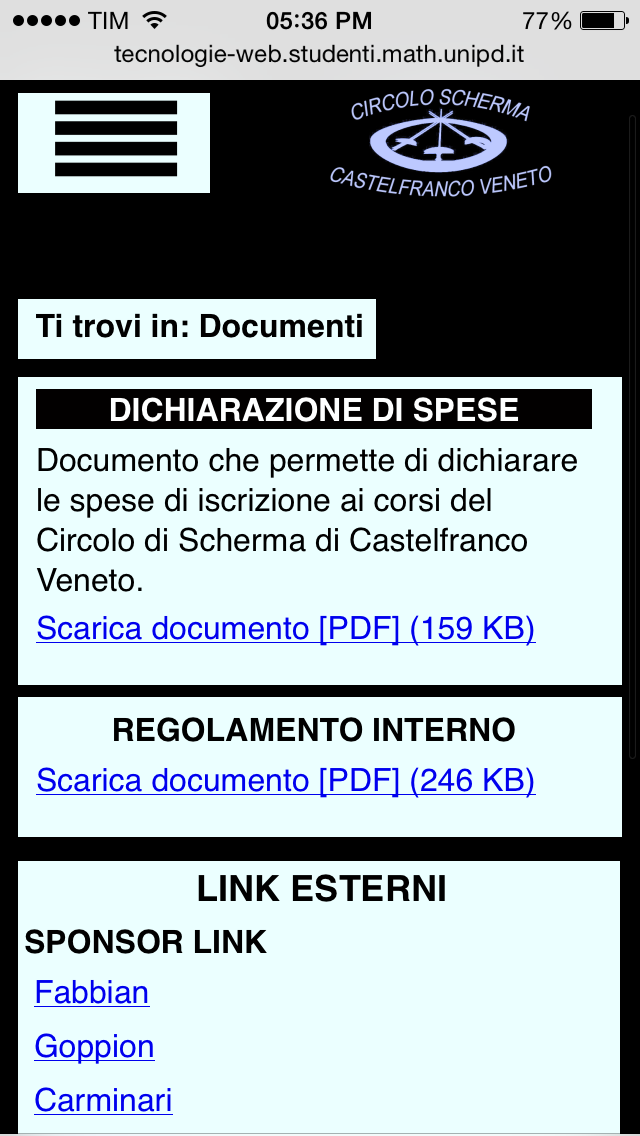
\includegraphics[scale=0.30]{images/articoli_mobile.png}
%		\caption{Screenshot mobile articoli.cgi}
%        \end{subfigure}
%        \caption{Layout schermi diversi}\label{layout}
%\end{figure}

Sono previste inoltre delle variazione del layout nel caso javascript sia disabilitato nel browser client. In particolare nelle pagine di inserimento o modifica della parte amministratore, vengono nascosti i bottoni dei tag speciali e la sidebar con la legenda, per far spazio ad una colonna con le istruzioni per inserire i tag correttamente.
\`E previsto inoltre uno stile per internet explorer 8 e precedenti, che semplifica la disposizione degli elementi attivando lo stile tablet, in modo da rendere il ridimensionamento della finestra fluido e senza problemi.

%\begin{figure}[h!]
%        \centering
%        \begin{subfigure}[b]{0.48\textwidth}
%                \includegraphics[width=\textwidth]{images/formJavascript.png}
%                \caption{javaScript abilitato}
%                \label{javascript}
%        \end{subfigure}
%        ~
%        \begin{subfigure}[b]{0.48\textwidth}
%                \includegraphics[width=\textwidth]{images/formNoJavascript.png}
%                \caption{javaScript disabilitato}
%                \label{nojavascript}
%        \end{subfigure}
%        \caption{Layout con/senza javascript}\label{layoutJavascript}
%\end{figure}
	\subsection{Scelte implemetative}
		\subsubsection{Gestione amministrazine mobile}
Per quanto riguarda la parte amministrativa si \`e scelto di non permetterne la gestione nei dispositivi mobile in quanto ritenuta scomoda e poco pratica. \\
 L'accesso all'area privata sar\`a dunque possibile solo da tablet e da desktop.

\subsubsection{Nota su inserimento articoli e documenti}
Si \`e scelto di supporre che non possano essere inseriti articoli avente stesso luogo e stessa data. Questa decisione deriva dal fatto che il gestore del sito ci ha informato che non si \`e mai verificato questo conflitto.
\\ La stessa considerazione \`e stata fatta per i documenti, i quali non possono avere lo stesso titolo.
\newpage
\section{Accessibilit\`a}
	\subsection{Link nascosti}
Per rendere il sito pi\`u accessibile e migliorare la navigazione, in particolar modo per le persone non vedenti o comunque per tutti coloro che utilizzano come supporto uno screen reader, abbiamo deciso di introdurre numerosi link nascosti che consentono di muoversi agilmente all'interno di una determinata pagina web. \\
Ecco nel dettaglio la loro implementazione:
	\begin{itemize}
		\item \textbf{Salta men\`u di navigazione}: questo link ti permette di saltare il men\`u principale e posizionarti prima del breadcrumb in modo che l'utente possa ricordarsi dove si trova e poi leggere il contenuto della pagina. Questo aiuto ti informa anche che se salti quest'area della pagina salterai anche il link per accedere alla parte riservata all'amministrazione;
		\item \textbf{Salta contenuto}: questo collegamento serve se si ha la necessit\`a di andare alla sidebar perch\'e si vuole entrare in qualche sito correlato con il Circolo di Scherma o per visitare la Gallery per quanto riguarda la parte pubblica, mentre per la parte amministrativa ti consente di andare alla spiegazione di alcuni elementi per l'inserimento del testo nella form;
		\item \textbf{Torna su al men\`u di navigazione}: se si \`e letto tutto il contenuto o si ha superato la sidebar \`e possibile tornare al men\`u di navigazione per muoversi su altre pagine;
		\item \textbf{Torna al primo articolo/documento della pagina}: solo per le pagine che mostrano gli articoli e i documenti presenti \`e stata impostata una scorciatoia che ti permette di tornare al primo articolo/documento presente nel contenuto.
 
	\end{itemize}
Per tornare su all'inizio del contenuto per chi non utilizza screen reader \`e stato inserito un torna su unico situato in basso a destra che si attiva solo quando si \`e scorso la pagina.
\\ Il meccanismo viene gestito tramite javascript, ma se viene disabilitato allora vengono resi disponibili a tutti gli utenti le scorciatoie previste per i non vedenti. \\
\\ Per capire se i link siano stati inseriti in zone utili, abbiamo provato ad utilizzare il sito disabilitando gli stili. Inoltre ci siamo avvalsi del plugin Fangs per vedere come il sito viene visto da uno screen reader e ci\`o che appare sembra conforme alle necessit\`a di una persona con disabilit\`a in particolare visive.
\subsection{Lista nascosta}
Per facilitare la navigazione tra gli articoli e i documenti \`e stata inserita una lista nascosta di link (prima del contenuto) che rimandano al testo esatto selezionato.

\subsection{Tab Index}
Un altro meccanismo utilizzato per consentire una migliore esperienza per l'utente \`e stato quello di personalizzare i tab index in modo che ci si possa muovere pi\`u velocemente e senza avere bisogno del mouse.
In particolare gli abbiamo utilizzati per la navigazione nel men\`u e per i form presenti nella parte amministrativa.

\subsection{Breadcrumb}
Per far capire all'utente in che sezione del sito si trova, abbiamo pensato di modificare il colore di sfondo nella lista del menu\`per la pagina selezionata. La scelta di usare questo metodo  per veicolare questa informazione \`e stata scelta per eleganza, ma confermata da un'analisi del contrasto dei colori che rende ci\`o accessibile anche a chi ha particolari problemi di vista che analizzeremo nel capitolo successivo.
\\  Per chi utilizza screen reader è stato invece predisposto un campo nascosto che ti dice dove sei.
\\ Questo campo diventa visibile anche a tutti gli utenti quando si passa in modalità tablet e mobile in quanto il men\`u viene compresso e quindi non \`e pi\`u intuibile capire dove si \`e.

\subsection{Contrasti dei colori}
Per verificare che ci sia il giusto contrasto tra i colori applicati al sito abbiamo utilizzato due strumenti consigliati a lezione: Colour Contrast Analyser e Vischeck.
Abbiamo fatto due tipi di test, uno relativo al giusto contrasto tra il testo e lo sfondo e uno riguardante le possibile difficolt\`a che possono riscontrare utenti affetti da alcune distorsioni visive su una generica pagina del sito.
	\subsubsection {Test - Contrasto testo e sfondo}
	Questo tipo di test \`e  stato effettuato con Colour Contrast Analyser e si riscontrano i seguenti risultati:
	\\ Il contrasto risultante del colore azzurro chiaro (ebffff) di sfondo e nero come testo ha superato tutti i test presenti nell'applicazione.
	\\ L'analisi della \textbf{differenza colore/luminosit\`a} per una visione normale da risultati (745/249) con soglia minima fissata per superare il test a 500. Anche per chi soffre di alcuni distrubi della vista* i test sono superati con un minimo margine, ma sufficiente a garantirne l'accessibilit\`a.
	\\ Anche l'analisi \textbf{della luminosit\`a} risulta positiva a tutte le prove con rapporto di contrasto 20.3:1, con soglia minima perchè tutti i test siano validi fissata a 7:1, per chi vede normalmente la pagina. Rimane un rapporto alto anche per chi soffre di alcuni disturbi della vista* compreso tra i (17.3 e 19.9):1.
	\\
	\\
	\\Il contrasto risultante del colore blu di sfondo e bianco come testo usato nel men\`u di navigazione ha superato tutti i test presenti nell'applicazione.
	\\ L'analisi della \textbf{differenza colore/luminosit\`a} per una visione normale da risultati (543/212) con soglia minima fissata per superare il test a 500. Anche per chi soffre di alcuni distrubi della vista* i test sono superati con un discreto margine.
	\\ Anche l'analisi \textbf{della luminosit\`a} risulta positiva a tutte le prove con rapporto di contrasto 10.9:1, con soglia minima perchè tutti i test siano validi fissata a 7:1, per chi vede normalmente la pagina. Rimane comunque a un buon rapporto compreso tra i (9.7 e 14.4):1 per chi soffre di alcuni disturbi della vista*.
	\\
	\\
	\\Sono stati analizzati anche i contrasti con i colori dei link (normale,visitato) con lo sfondo azzurrino.
	\\Per quanto riguarda questi link, sia l'analisi della differenza colore/luminosit\`a sia quella della luminosit\`a,  vengono superate. In alcuni casi e per alcune distorsioni con una soglia minima, mentre per altri con un ampio margine.
	\\ \\ \textbf{*Disturbi della vista testati}: daltonismo, protanopia, tritanopia, deuteranopia.

	\subsubsection {Test - Distorsioni visive}
	Il sequente test invece \`e  stato effettuato attraverso il sito web Vischeck e si riscontrano i seguenti risultati:
	\begin{itemize}
	\item Per chi soffre di \textbf{deuteranopia}, cio\`e chi confonde il rosso porpora con il verde, in figura \ref{deuteranopia} ci\`o che appare:
	
	\item Per chi soffre di \textbf{pronatopia}, cio\'e una forma di daltonismo per i colori rosso e verde,  in figura \ref{protanopia} ci\`o che appare:
	
	\item Per chi soffre di \textbf{tritanopia}, cio\`e cecit\`a per il blu e il violetto, in figura \ref{tritanopia} ci\`o che appare:
	\end{itemize}
	
	\begin{figure}[h!]
		\centering
		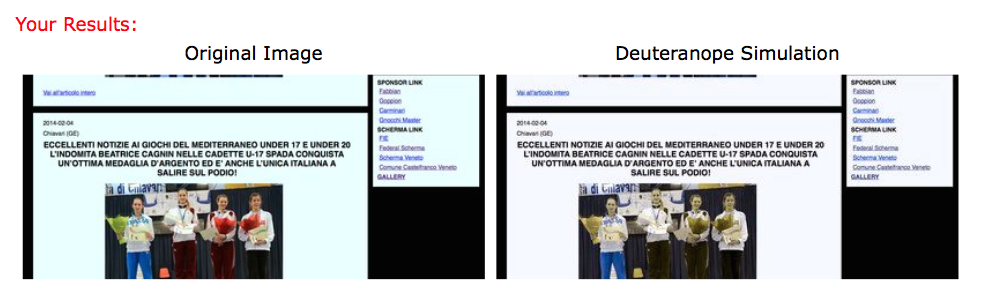
\includegraphics[scale=0.4]{images/contrasto_pagina_deuteranope.png}
		\caption{Visualizzazione sito per chi soffre di deuteranopia}
		\label{deuteranopia}
	\end{figure}	
	
	\begin{figure}[h!]
		\centering
		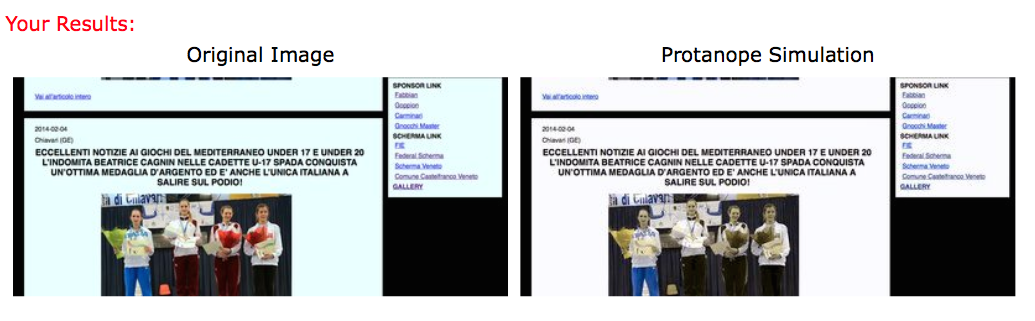
\includegraphics[scale=0.4]{images/contrasto_pagina_protanope.png}
		\caption{Visualizzazione sito per chi soffre di protanopia}
		\label{protanopia}
	\end{figure}
	
	\begin{figure}[h!]
		\centering
		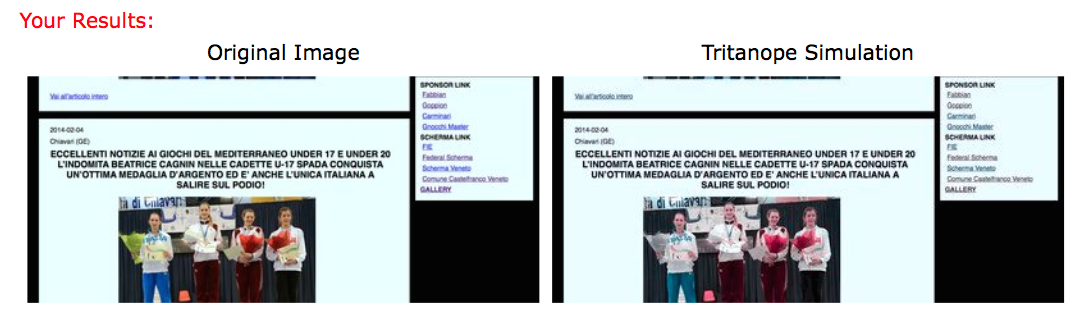
\includegraphics[scale=0.4]{images/contrasto_pagina_tritanope.png}
		\caption{Visualizzazione sito per chi soffre di tritanopia}
		\label{tritanopia}
	\end{figure}
	\newpage
	\textbf{Conclusioni}: per tutti e tre i tipi di distorsione il contrasto che si ottiene fa si che l'utente riesca comunque a comprendere il contenuto e a orientarsi nella pagina riuscendo ad interpretare il men\`u e i link presenti.

\subsection{Mappa del sito}
\`E stato scelto di non inserire una mappa in quanto il numero di pagine presenti nel sito \`e in numero ristretto e difficilmente l'utente potr\`a perdersi durante la navigazione.	

\newpage
\section{Validazione}
	\subsection{HTML5}
Tutte le pagine sono state create con il doctype di HTML5, sotto suggerimento della Professoressa,  per non avere pi\`u errori di validazione con i tag <noscript> e con l'attributo target dei link che portano ad altri siti.
\\ Abbiamo testato la validit\`a di tutte le pagine, attraverso il validatore \href{http://validator.nu}{http://validator.nu} in quanto il validatore del W3C al momento dei test non funzionva, con i seguenti risultati:
\begin{itemize}
	\item Per le pagine statiche staff.html, storia.html e errore.html la validazione \`e avvenuta con successo, mentre per quanto riguarda corsi.html si sono riscontrati degli errori sull'attributo summary del tag table in quanto in HTML5 viene considerato obsoleto e sull'attributo href del link alla gallery in quanto il carattere \& non \`e stato utilizzato per antecedere ad un carattere speciale. In seguito verranno spiegati i motivi che ci hanno fatto optare per non correggere tutti gli errori riscontrati.
	\item Per le pagine dinamiche della parte pubblica articoli.cgi e documenti.cgi vengono generate delle pagine che non validano solo per l'attributo id degli articoli e dei documenti in quanto contengono degli spazi.
	\\La pagina amministra.cgi invece genera una pagina valida;
	\item Per la pagina dinamica della parte privata: amministraSezionePrivata.cgi abbiamo validato tutte le singole pagine che venivano stampate in output dal browser a seconda dei diversi casi.
	\\ Queste vengono validate totalmente. 
\end{itemize}
L'omissione di alcuni errori \`e stata una scelta voluta in quanto si \`e deciso di permettere una maggiore accessibilit\`a a scapito di un possibile posizionamento migliore nei motori di ricerca.
\\  Questa decisione viene presa perch\`e la maggior parte degli utenti che visita il sito conosce gi\'a il link  e non va a caso nella ricerca. Inoltre il sito non contiene informazioni di carattere generale sulla scherma, quindi in una ricerca casuale non ha importanza che il sito sia visualizzato tra i primi risultati.

\subsection{CSS}
La validazione dei css \`e stata fatta attraverso il validatore 
\href{http://jigsaw.w3.org/css-validator}{http://jigsaw.w3.org/css-validator}
e per tutti i file: stile.css, print.css e stilenojava.css il risultato \`e stato positivo senza nemmeno un warning.
 
\subsection{XML e XSD}
La validazione dei file XML rispetto agli schemi corrispondenti \`e stata effettuata tramite il seguente validatore on-line:
\\
\href{http://www.freeformatter.com/xml-validator-xsd.html}{http://www.freeformatter.com/xml-validator-xsd.html}
\\Non è stato utilizzato il validatore del W3C poich\`e al momento non era funzionante.
\\La validazione ha avuto un risultato positivo per tutti i file.
	

\newpage
\section{Compatibilit\`a}
	Riportiamo di seguito, per ogni sistema operativo, i browser con cui abbiamo verificato la compatibilit\`a:
\begin{itemize}
		\item WINDOWS 7
		\begin{itemize}
			%\item IEXPLORER 6
			\item IEXPLORER 7
			\item IEXPLORER 8
			\item IEXPLORER 9
			\item CHROME 33
			\item FIREFOX 19
		\end{itemize}
		\item MAC OSx 10.9.2
		\begin{itemize}
			\item CHROME 33
			%\item OPERA 
			\item FIREFOX 27
			\item SAFARI 7
		\end{itemize}
		\item LINUX UBUNTU 12.04.3 LTS
		\begin{itemize}
			\item CHROME 33
			\item FIREFOX 24
			\item OPERA 12.16
		\end{itemize}
\end{itemize}

Sono stati riscontrati problemi con le versioni 7 e 8 di Internet Explorer poich\`e queste versioni del browser non supportano le media queries. Per questo motivo abbiamo creato dei fogli di stile appositamente per queste versioni.
\\Non abbiamo riscontrato problemi con i rimanenti browser.
\\Abbiamo fatto alcuni test di compatibilit\`a anche su IPAD 2 e IPHONE 5 con i seguenti browser:
\begin{itemize}
	\item SAFARI
	\item CHROME
\end{itemize}
senza riscontrare alcun problema.
\newpage
\section{Ruoli}
	Tutti i componenti del gruppo hanno partecipato generalemente in tutte le parti del progetto cercando di apprendere nuove conoscenze e strumenti. \\
Nello specifico:
\begin{itemize}
	\item Mirko Pavanello: back-end e gestione dati xml; 
	\item Chiara Bigarella: getioni dati xml, schemi xsd, alcune parti del back-end e validazione;
	\item Massimiliano Sartoretto: implementazioni controlli e funzionalit\`a javascript, fogli di trasformazione xsl;
	\item Paolo Tesser: parte responsive, css, alcune funzioni javascript, accessibilit\`a e validazione.
\end{itemize}
\end{document}